\documentclass[conference]{IEEEtran}
\IEEEoverridecommandlockouts

\usepackage{cite}
\usepackage{amsmath,amssymb,amsfonts}
\usepackage{algorithmic}
\usepackage{graphicx}
\usepackage{textcomp}
\usepackage{xcolor}
\def\BibTeX{{\rm B\kern-.05em{\sc i\kern-.025em b}\kern-.08em
    T\kern-.1667em\lower.7ex\hbox{E}\kern-.125emX}}

\begin{document}

\title{Conference Paper Title*}

\author{
\begin{center}
\begin{tabular}{cc}
\begin{tabular}{c}
\textbf{1\textsuperscript{st} Given Name Surname} \\
Dept. name of organization \\
Name of organization \\
City, Country \\
email1@example.com
\end{tabular}
&
\begin{tabular}{c}
\textbf{2\textsuperscript{nd} Given Name Surname} \\
Dept. name of organization \\
Name of organization \\
City, Country \\
email2@example.com
\end{tabular}
\\[3.5em]
\begin{tabular}{c}
\textbf{3\textsuperscript{rd} Given Name Surname} \\
Dept. name of organization \\
Name of organization \\
City, Country \\
email3@example.com
\end{tabular}
&
\begin{tabular}{c}
\textbf{4\textsuperscript{th} Given Name Surname} \\
Dept. name of organization \\
Name of organization \\
City, Country \\
email4@example.com
\end{tabular}
\end{tabular}
\end{center}
}

\maketitle


\begin{abstract}
This document is a model and instructions for \LaTeX.
This and the IEEEtran.cls file define the components of your paper [title, text, heads, etc.]. *CRITICAL: Do Not Use Symbols, Special Characters, Footnotes, 
or Math in Paper Title or Abstract.
\end{abstract}

\begin{IEEEkeywords}
component, formatting, style, styling, insert.
\end{IEEEkeywords}

\section{Introduction}

Cold storage has diverse applications over various industries. Fresh produce is kept in supermarkets on refrigeration racks to prevent thermal and bacterial spoilage, while raw products such as sashimi rely on cold storage to treat parasites in aquatic produce. In the medical industry, vaccines are stored under low temperatures to maintain antigen viability. The Pfizer-BioNTech vaccine
requires a storage temperature of -80 $^{\circ}$C due to thermal instability of mRNA and its encapsulating lipid nanoparticles as an example\cite{uddin_challenges_2021}. A large proportion of the products from these categorical examples are volatile under temperature changes, hence it is necessary to maintain temperature control throughout the product to consumer distribution chain. Cold storage during transport is often more costly than stationary storage due to lower energy efficiency, caused by variable ambient temperature and lower insulation \cite{maiorino_refrigerated_2021}, thus motivating a separate analysis of higher refrigeration costs in transport operations.\\
Additionally, cold chain transport produces greenhouse gases in the form of CO$_2$ and refrigerants in cases of leaks. Greenhouse gases are the primary cause of global warming and its subsequent effects of climate change, which includes but are not limited to an increased transmissibility of tropical diseases \cite{thomson_climate_2022} and crop failure due to floods \cite{mirza_climate_2011}. In accordance to decision making associated with 
corporate social responsibility and the UN SDG 13 (Climate Action), it is important to reduce the effects of cold chain transport to the climate and external stakeholders, motivating the analysis of variables affecting  transport emissions.\\
We thus propose a model which aims to optimize transport costs, emissions, and customer satisfaction from a cold chain consisting of transport from suppliers to customers by employing Mixed Integer Linear Programming with Coin Branch and Cut and LSGA-2. The cold chain model is integrated with a customer satisfaction variable in order to reflect the importance of timeliness  in transport to customers.

\bigskip

\section{Literature Review}

The optimization of cold-chain logistics networks has become critical in balancing cost, carbon emissions, and service quality. Liu et al. (2021) develop an integer‐programming model for “origin–DC–customer” routing of fresh products, explicitly incorporating energy‐saving and emission‐reduction objectives alongside inventory, damage, penalty, and refrigeration costs \cite{Liu2021} (Liu et al., 2021). They compare a pure genetic algorithm with a hybrid GA–local‐search approach on real‐world data, demonstrating that the hybrid method yields superior Pareto‐front solutions for total cost and emissions.\\
For strategic facility location, Li and Zhou (2021) propose a multi‐objective mixed‐integer programming model for cold‐chain distribution center siting that integrates dynamic transportation emissions, static DC emissions, construction and operation costs, and time‐window penalty costs for customer satisfaction \cite{Li2021} (Li & Zhou, 2021). Their work employs NSGA-II, leveraging fast non‐dominated sorting and elitist selection, to generate diverse Pareto‐optimal trade-offs between cost, emissions, and service level.\\
The use of evolutionary multi‐objective algorithms in cold‐chain design is well established. Deb et al. (2002) introduced NSGA-II—now a de facto standard for handling complex, non‐convex multi‐criteria problems—which Li and Zhou adopt to efficiently explore large solution spaces under conflicting objectives \cite{Deb2002} (Deb et al., 2002). Complementing this, Ehrgott (2005) surveys multi‐criteria optimization methods, providing theoretical foundations for interpreting Pareto‐frontiers and supporting decision‐maker preference elicitation in supply‐chain contexts \cite{Ehrgott2005} (Ehrgott, 2005).\\
Carbon‐emission accounting in logistics has evolved from static factor models to more granular, load‐dependent formulations. Min and Zhou (2002) incorporate per‐km emission factors and load ratios into location‐allocation decisions, an approach echoed in Liu et al.'s refrigerated‐vehicle emission terms and Li and Zhou’s dynamic‐static emission splits \cite{Min2002} (Min & Zhou, 2002). Macharis et al. (2009) further distinguish fixed DC emissions from transport emissions, justifying the separate $\theta S_i$ and $\chi$-terms in our model’s carbon objective \cite{Macharis2009} (Macharis et al., 2009).\\
Time‐window constraints and service‐level penalties are classical in vehicle routing. Solomon (1987) formalizes VRPTW with soft and hard time windows, introducing early/late penalties analogous to our piecewise cost function $C(T_{jk})$ \cite{Solomon1987} (Solomon, 1987). Savelsbergh and Sol (1995) review exact and heuristic VRPTW methods, offering practical insights into penalty‐incorporating routing heuristics that inform both Liu et al.’s and Li and Zhou’s solution algorithms \cite{Savelsbergh1995} (Savelsbergh & Sol, 1995).\\
Recent research extends the integration of cold-chain logistics with sustainability goals. Wang et al. (2023) present a green vehicle routing model that incorporates battery electric trucks with limited range and recharging constraints, balancing carbon footprint reduction with cost and time penalties \cite{Wang2023} (Wang et al., 2023). Similarly, Chen and Huang (2022) develop a stochastic multi‐objective framework for cold-chain distribution under demand uncertainty, employing a robust optimization approach to hedge against variability while maintaining carbon and cost efficiency \cite{Chen2022} (Chen & Huang, 2022).\\
The rise of IoT and real-time monitoring technologies also offers new avenues to enhance cold-chain efficiency. For instance, Silva et al. (2021) integrate sensor data for real-time temperature and location tracking to dynamically adjust routing and storage decisions, minimizing spoilage risks and energy consumption \cite{Silva2021} (Silva et al., 2021). These data-driven approaches complement traditional optimization, enabling adaptive and more resilient logistics networks.\\
Finally, decision-support systems increasingly incorporate interactive multi-criteria decision analysis (MCDA) tools to facilitate stakeholder engagement in cold-chain planning. Brans and Mareschal (2005) demonstrate the application of PROMETHEE methods to balance environmental and economic objectives, providing transparent trade-off visualization to decision-makers \cite{Brans2005} (Brans & Mareschal, 2005). This human-in-the-loop perspective is vital given the complexity and competing priorities in cold-chain logistics.

\bigskip

\section{Problem Formulation}

In our problem formulation, we have a set of $I$ supplier, $J$ distribution centers (DCs), and $K$ customers, which can be thought of as supermarkets or stores.
We act as both the suppliers and distributors of a product, starting without any distribution centers initially. The goal is to transport the goods while optimizing for the costs, carbon emissions, and customer utilitiy. As we have multiple objective functions, we often have to optimize for the best compromise  \cite{benayounLinearProgrammingMultiple1971}, as an optimal solution for all might not exist. \\
There are costs associated with acting as bost supplier and distributor. First, the distribution 
centers must be built, if they haven't already. This has a cost associated per unit of area. Note that we can include the cost of buying the land into this if required, and we note we can set the costs as 0 if we already own the distribution centers.
Next, there is also a cost associated with running the distribution facilities. This is proportional to the size of the facility. Although costs might vary per distribution center, we assume for simplicity that the costs are flat per unit of area. Finally, we also assume for simplicity we have infinite trucks to transport the goods. \\
There is also a cost associated with transporting te goods from the supply center to the distribution center, then from the distribution center to the customer. This is proportional to the number of trucks required, the distance between the locations, and the cost of transporting per km.\\
Finally, goods can be damaged in transport. We represent this as opportunity cost, as we can't sell damaged goods. The cost is proportional to the price of the object, the damage rate per km, as different objects could have different rates, and the distance traveled.\\
For carbon costs, it is proportional to the carbon efficiency of the vehicle (measured for example as carbon emissions / km), how far we must travel, and how full the truck, as more weight could result in more emissions \cite{du_plessis_calculating_2023}. Note we assume that all the trucks must return to their original individual supply centers, and so in one way there is the cost associated with the weight, but in the other the truck is empty.\\
Customer satisfaction is proportional to the arrival of the vehicles to the customer. If they are within a reasonable tolerance, it incurs no penalty. But if the vehicle arrives too late or too early, we incur a penalty proportional to how late or early we are.
\subsection*{Sets}
\begin{itemize}
    \item $I$ : Set of suppliers
    \item $J$ : Set of distribution centers (DCs)
    \item $K$ : Set of customers
\end{itemize}

\subsection*{Parameters}
\begin{itemize}
    \item $d_{ij}$ : Distance from supplier $i$ to DC $j$
    \item $d_{jk}$ : Distance from DC $j$ to customer $k$
    \item $N_k$ : Demand of customer $k$
    \item $s_j$ : Area required for DC $j$
    \item $z$ : Construction cost per unit area
    \item $w$ facility cost per unit area
    \item $e$ : Unit value of goods
    \item $u$ : Damage rate per km
    \item $\delta$ : Transport cost per truck per km
    \item $\rho_{\max}, \rho_0$ : Fuel consumption per km (full/empty)
    \item $\chi$ : Carbon cost of vehicle per km
    \item $\theta$ : Static carbon cost coefficient
    \item $\phi$ : CO$_2$ conversion per unit goods
    \item $Q$ : Maximum vehicle load
    \item $\alpha_1, \alpha_2$ : Penalty coefficients for early/late delivery
    \item $RT_k, LT_k$ : Time window boundaries for customer $k$
    \item $U$ : Maximum penalty cost
    \item $\eta^{\max}_j$ : Maximum number of vehicles allowed at DC $j$
    \item $S_i$: Maximum storage for DC $i$
\end{itemize}

\subsection*{Decision Variables}
\begin{itemize}
    \item $c_j \in \{0,1\}$ : 1 if distribution center $j$ is opened
    \item $x_{ij} \in \{0,1\}$ : 1 if supplier $i$ supplies DC $j$
    \item $y_{jk} \in \{0,1\}$ : 1 if DC $j$ serves customer $k$
    \item $t_{ij} \geq 0$ : Quantity of goods transported from supplier $i$ to DC $j$
    \item $t_{jk} \geq 0$ : Quantity of goods transported from DC $j$ to customer $k$
    \item $T_{jk} \geq 0$ : Arrival time at customer $k$ from DC $j$
    \item $\eta_j \in \mathbb{Z}_+ \quad$ : Number of vehicles allocated to DC $j$
\end{itemize}

\subsection*{Objective Functions}
\subsection*{1. Costs ($C_c$)}
\begin{align}
\min C_c = &\sum_{j \in J} c_j (z s_j + w s_j) \\
&+ \delta \sum_{i \in I} \sum_{j \in J} x_{ij} \lceil \frac{t_{ij}}{Q}\rceil d_{ij}
+ \delta \sum_{j \in J} \sum_{k \in K} y_{jk} \lceil \frac{t_{jk}}{Q} \rceil d_{jk} \nonumber \\
&
+ e \sum_{i \in I} \sum_{j \in J} x_{ij} u d_{ij}
+ e \sum_{j \in J} \sum_{k \in K} y_{jk} u d_{jk} \nonumber
\end{align}

\subsection*{2. Carbon Emission Cost ($T_c$)}
\begin{align}
\min T_c = &\theta S_i+ \sum_{j \in J} c_j \phi \sum_{i \in I} t_{ij} \\
&+ \chi \sum_{i \in I} \sum_{j \in J} x_{ij} \left(
\frac{\rho_{\max} - \rho_0}{Q} t_{ij} d_{ij} + \rho_0 d_{ij}
\right) \nonumber \\
&+ \chi \sum_{j \in J} \sum_{k \in K} y_{jk} \left(
\frac{\rho_{\max} - \rho_0}{Q} t_{jk} d_{jk} + \rho_0 d_{jk}
\right) \nonumber
\end{align}

\subsection*{3. Customer Satisfaction Penalty Cost ($U_c$)}
\[
\min U_c = \sum_{j \in J} \sum_{k \in K} y_{jk} \cdot C(T_{jk})
\]
Where:
\[
C(T_{jk}) =
\begin{cases}
\alpha_1 (RT_k - T_{jk}), & T_{jk} < RT_k \\
0, & RT_k \leq T_{jk} \leq LT_k \\
\alpha_2 (T_{jk} - LT_k), & LT_k < T_{jk} \\
\end{cases}
\]

\subsection*{Constraints}
\begin{align}
t_{ij}, t_{jk} &\geq 0 \quad \forall i,j,k \\
\sum_{i \in I} t_{ij} &= \sum_{k \in K} t_{jk} \quad \forall j \\
\sum_{j \in J} c_j &\geq 1 \\
\sum_{k \in K} t_{jk} &\leq \eta_j \cdot Q \quad \forall j \\
\sum_{j \in J} t_{jk} &= N_k \quad \forall k \\
c_j, x_{ij}, y_{jk} &\in \{0, 1\} \quad \forall i,j,k \\
0 \leq \eta_j &\leq \eta_j^{\max} \quad \forall j
\end{align}

\bigskip

\section{Variable Choices}
Variables chosen are based on quantitative data done by the research of . Numerical values of the variables are given as following :
\begin{center}
\resizebox{\linewidth}{!}{
\begin{tabular}{@{}llp{5cm}l@{}}
    \toprule
    Variable & Description & Value & Source\\
    \midrule
    $\rho_{\max}$ & Fuel consumption under maximum weight & 2.0610 l/km & \cite{du_plessis_calculating_2023}\\ 
    $\rho_0$ & Fuel consumption under zero load  & 0.3744 l/km & \cite{du_plessis_calculating_2023}\\
    $\chi$ & Carbon cost of vehicle per kilometer & Average fuel consumption * CO$_2$ emissions per kilometer = 1.3909 kg $CO_2e/km$ & \cite{du_plessis_calculating_2023}\\ 
    $\phi$ & CO$_2$ conversion per unit goods & 0.87-1.28 kg CO$_2$e/kg & \cite{plessis_energy_2024}\\
    $\theta$ & Static Carbon Cost Coefficient & 0.190 USD/kg & \cite{iwg_scghg_2021}\\
\end{tabular}
}
\end{center}

\bigskip

\subsection{Equations}
Number equations consecutively. To make your 
equations more compact, you may use the solidus (~/~), the exp function, or 
appropriate exponents. Italicize Roman symbols for quantities and variables, 
but not Greek symbols. Use a long dash rather than a hyphen for a minus 
sign. Punctuate equations with commas or periods when they are part of a 
sentence, as in:
\begin{equation}
a+b=\gamma\label{eq}
\end{equation}

Be sure that the 
symbols in your equation have been defined before or immediately following 
the equation. Use ``\eqref{eq}'', not ``Eq.~\eqref{eq}'' or ``equation \eqref{eq}'', except at 
the beginning of a sentence: ``Equation \eqref{eq} is . . .''

\subsection{\LaTeX-Specific Advice}

Please use ``soft'' (e.g., \verb|\eqref{Eq}|) cross references instead
of ``hard'' references (e.g., \verb|(1)|). That will make it possible
to combine sections, add equations, or change the order of figures or
citations without having to go through the file line by line.

Please don't use the \verb|{eqnarray}| equation environment. Use
\verb|{align}| or \verb|{IEEEeqnarray}| instead. The \verb|{eqnarray}|
environment leaves unsightly spaces around relation symbols.

Please note that the \verb|{subequations}| environment in {\LaTeX}
will increment the main equation counter even when there are no
equation numbers displayed. If you forget that, you might write an
article in which the equation numbers skip from (17) to (20), causing
the copy editors to wonder if you've discovered a new method of
counting.

{\BibTeX} does not work by magic. It doesn't get the bibliographic
data from thin air but from .bib files. If you use {\BibTeX} to produce a
bibliography you must send the .bib files. 

{\LaTeX} can't read your mind. If you assign the same label to a
subsubsection and a table, you might find that Table I has been cross
referenced as Table IV-B3. 

{\LaTeX} does not have precognitive abilities. If you put a
\verb|\label| command before the command that updates the counter it's
supposed to be using, the label will pick up the last counter to be
cross referenced instead. In particular, a \verb|\label| command
should not go before the caption of a figure or a table.

Do not use \verb|\nonumber| inside the \verb|{array}| environment. It
will not stop equation numbers inside \verb|{array}| (there won't be
any anyway) and it might stop a wanted equation number in the
surrounding equation.

\subsection{Some Common Mistakes}\label{SCM}
\begin{itemize}
\item The word ``data'' is plural, not singular.
\item The subscript for the permeability of vacuum $\mu_{0}$, and other common scientific constants, is zero with subscript formatting, not a lowercase letter ``o''.
\item In American English, commas, semicolons, periods, question and exclamation marks are located within quotation marks only when a complete thought or name is cited, such as a title or full quotation. When quotation marks are used, instead of a bold or italic typeface, to highlight a word or phrase, punctuation should appear outside of the quotation marks. A parenthetical phrase or statement at the end of a sentence is punctuated outside of the closing parenthesis (like this). (A parenthetical sentence is punctuated within the parentheses.)
\item A graph within a graph is an ``inset'', not an ``insert''. The word alternatively is preferred to the word ``alternately'' (unless you really mean something that alternates).
\item Do not use the word ``essentially'' to mean ``approximately'' or ``effectively''.
\item In your paper title, if the words ``that uses'' can accurately replace the word ``using'', capitalize the ``u''; if not, keep using lower-cased.
\item Be aware of the different meanings of the homophones ``affect'' and ``effect'', ``complement'' and ``compliment'', ``discreet'' and ``discrete'', ``principal'' and ``principle''.
\item Do not confuse ``imply'' and ``infer''.
\item The prefix ``non'' is not a word; it should be joined to the word it modifies, usually without a hyphen.
\item There is no period after the ``et'' in the Latin abbreviation ``et al.''.
\item The abbreviation ``i.e.'' means ``that is'', and the abbreviation ``e.g.'' means ``for example''.
\end{itemize}
An excellent style manual for science writers is .

\subsection{Authors and Affiliations}\label{AAA}
\textbf{The class file is designed for, but not limited to, six authors.} A 
minimum of one author is required for all conference articles. Author names 
should be listed starting from left to right and then moving down to the 
next line. This is the author sequence that will be used in future citations 
and by indexing services. Names should not be listed in columns nor group by 
affiliation. Please keep your affiliations as succinct as possible (for 
example, do not differentiate among departments of the same organization).

\subsection{Identify the Headings}\label{ITH}
Headings, or heads, are organizational devices that guide the reader through 
your paper. There are two types: component heads and text heads.

Component heads identify the different components of your paper and are not 
topically subordinate to each other. Examples include Acknowledgments and 
References and, for these, the correct style to use is ``Heading 5''. Use 
``figure caption'' for your Figure captions, and ``table head'' for your 
table title. Run-in heads, such as ``Abstract'', will require you to apply a 
style (in this case, italic) in addition to the style provided by the drop 
down menu to differentiate the head from the text.

Text heads organize the topics on a relational, hierarchical basis. For 
example, the paper title is the primary text head because all subsequent 
material relates and elaborates on this one topic. If there are two or more 
sub-topics, the next level head (uppercase Roman numerals) should be used 
and, conversely, if there are not at least two sub-topics, then no subheads 
should be introduced.

\subsection{Figures and Tables}\label{FAT}
\paragraph{Positioning Figures and Tables} Place figures and tables at the top and 
bottom of columns. Avoid placing them in the middle of columns. Large 
figures and tables may span across both columns. Figure captions should be 
below the figures; table heads should appear above the tables. Insert 
figures and tables after they are cited in the text. Use the abbreviation 
``Fig.~\ref{fig}'', even at the beginning of a sentence.

\begin{table}[htbp]
\caption{Table Type Styles}
\begin{center}
\begin{tabular}{|c|c|c|c|}
\hline
\textbf{Table}&\multicolumn{3}{|c|}{\textbf{Table Column Head}} \\
\cline{2-4} 
\textbf{Head} & \textbf{\textit{Table column subhead}}& \textbf{\textit{Subhead}}& \textbf{\textit{Subhead}} \\
\hline
copy& More table copy$^{\mathrm{a}}$& &  \\
\hline
\multicolumn{4}{l}{$^{\mathrm{a}}$Sample of a Table footnote.}
\end{tabular}
\label{tab1}
\end{center}
\end{table}

\begin{figure}[htbp]
\centerline{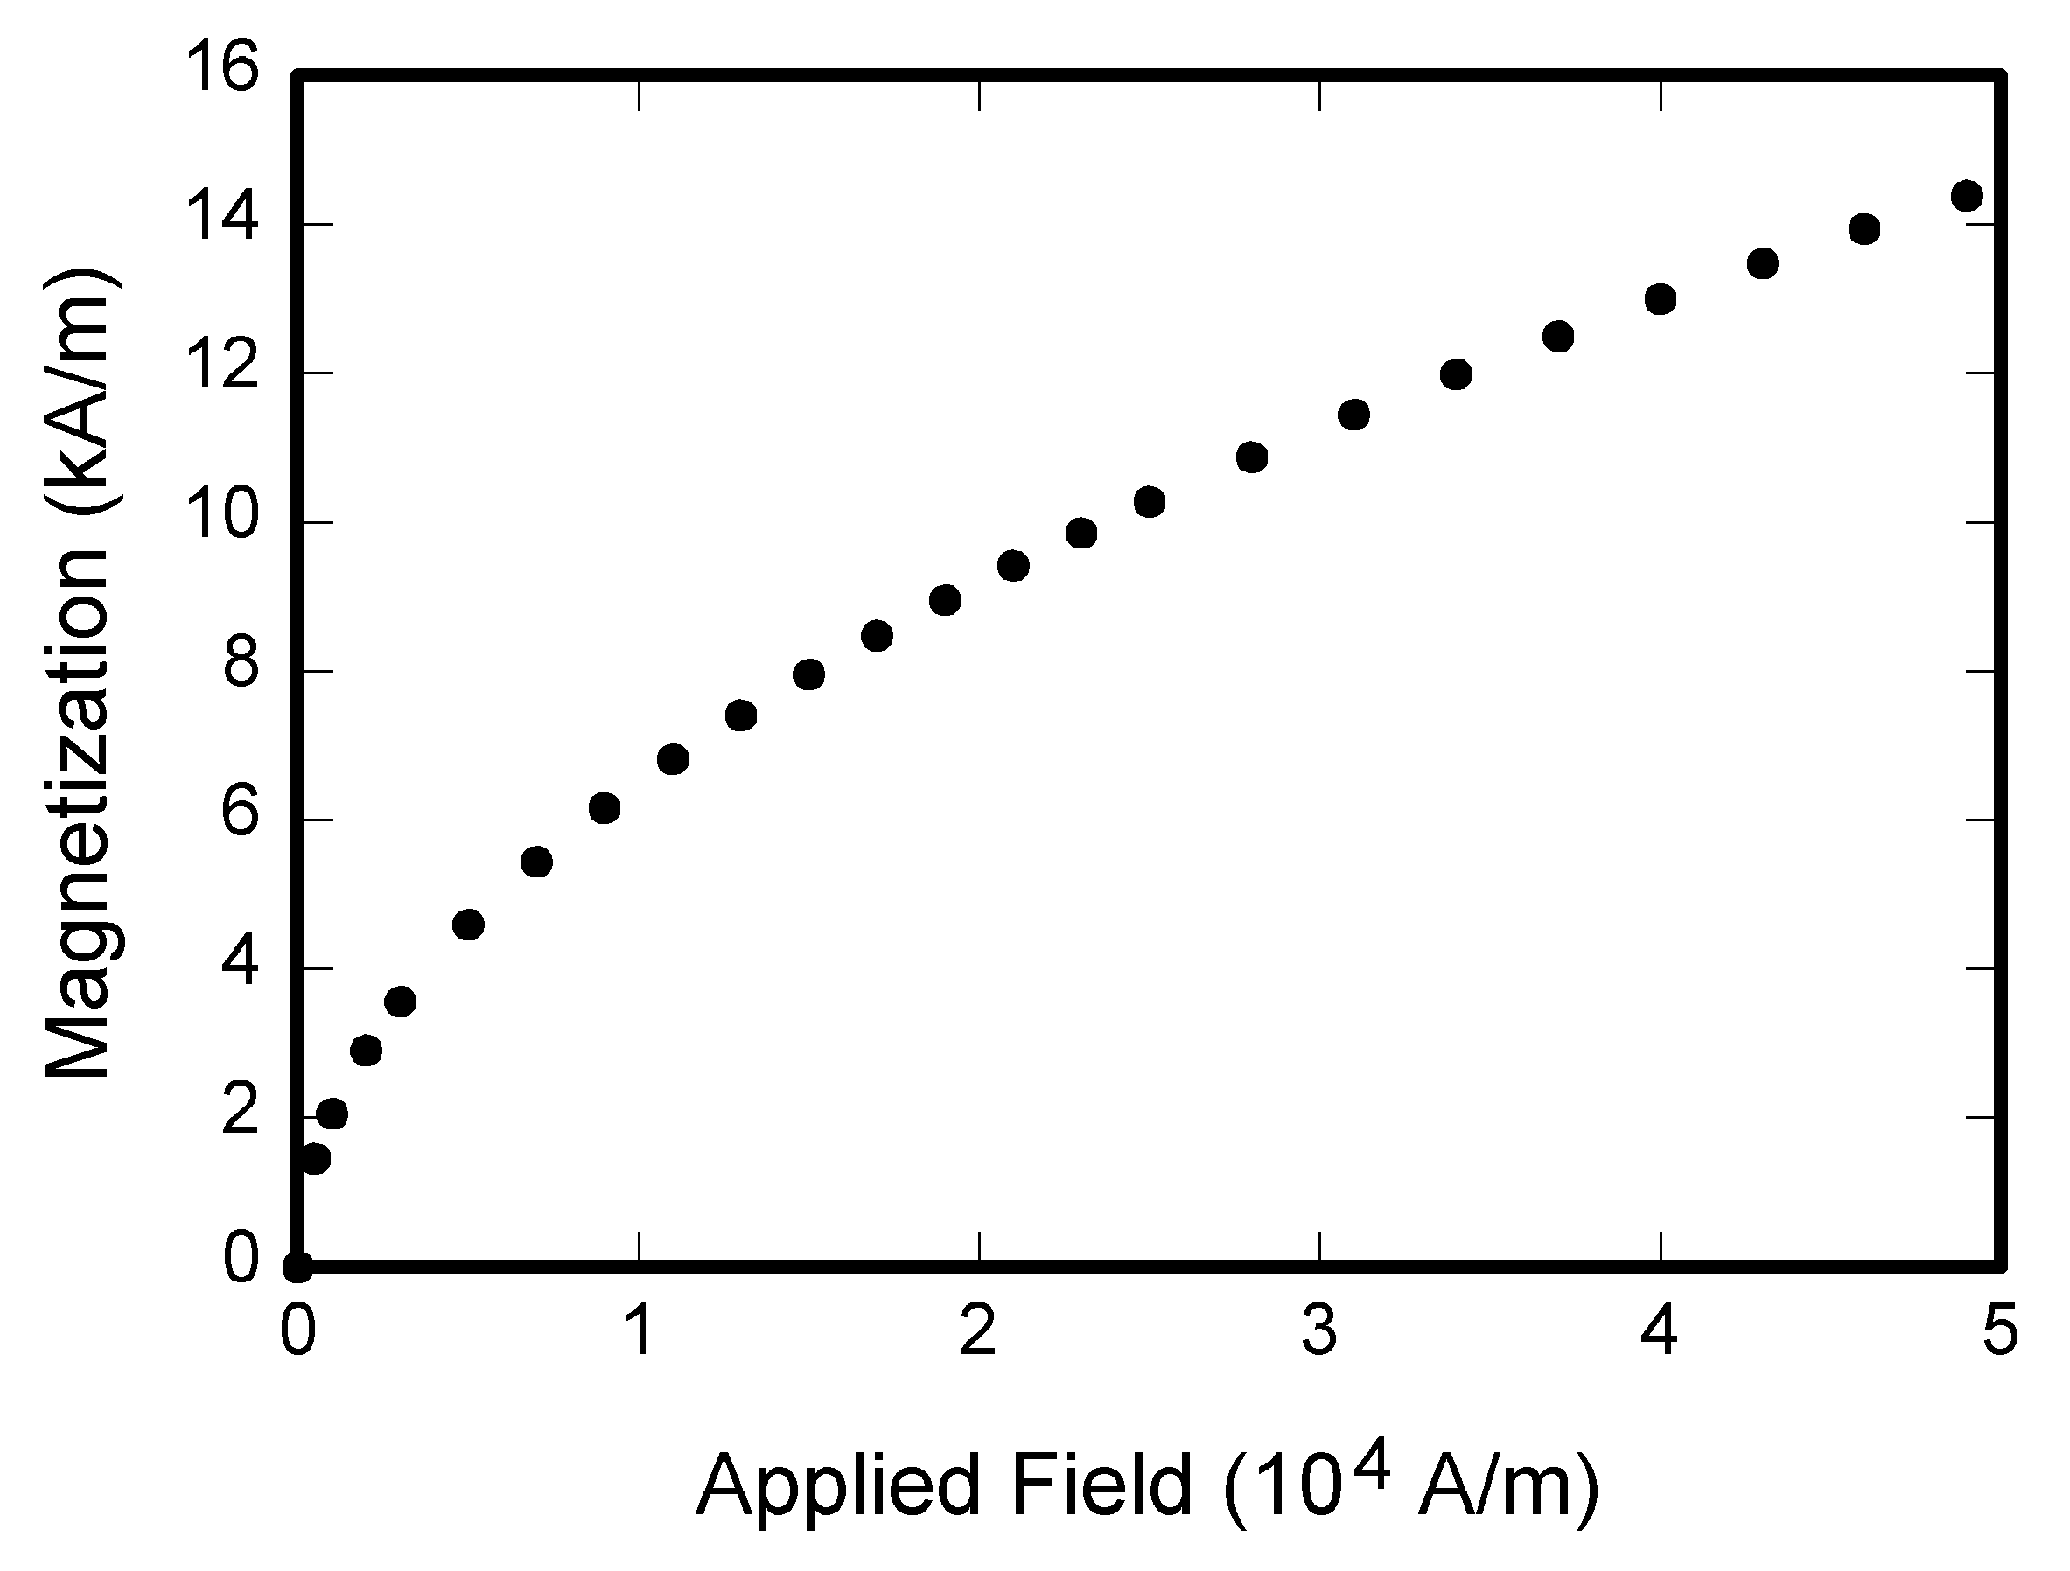
\includegraphics{fig1.png}}
\caption{Example of a figure caption.}
\label{fig}
\end{figure}

Figure Labels: Use 8 point Times New Roman for Figure labels. Use words 
rather than symbols or abbreviations when writing Figure axis labels to 
avoid confusing the reader. As an example, write the quantity 
``Magnetization'', or ``Magnetization, M'', not just ``M''. If including 
units in the label, present them within parentheses. Do not label axes only 
with units. In the example, write ``Magnetization (A/m)'' or ``Magnetization 
\{A[m(1)]\}'', not just ``A/m''. Do not label axes with a ratio of 
quantities and units. For example, write ``Temperature (K)'', not 
``Temperature/K''.

\section*{Acknowledgment}

The preferred spelling of the word ``acknowledgment'' in America is without 
an ``e'' after the ``g''. Avoid the stilted expression ``one of us (R. B. 
G.) thanks $\ldots$''. Instead, try ``R. B. G. thanks$\ldots$''. Put sponsor 
acknowledgments in the unnumbered footnote on the first page.

\bibliographystyle{IEEEtran}
\bibliography{AMMPaper}
\end{document}
